\documentclass[12pt]{dissertation} 

%load any additional packages
\usepackage[utf8]{inputenc} % Lets me include the reference to Škrbina N
\usepackage[bmargin=1.5in, margin=1.2in]{geometry}
\setlength{\footskip}{50pt}
\usepackage{amssymb}
\usepackage{natbib}
\usepackage{tikz}
\usepackage{url}
\usepackage{titlesec}
\usepackage[]{algorithm2e}
\usepackage{amsmath,amsfonts,amssymb,amsthm,bm}
\usepackage{caption}
\usepackage{wrapfig}
\usepackage{fancyvrb}
\usepackage{subcaption}
\usepackage{tikzscale}
\usepackage{multicol}
\usepackage[capitalise]{cleveref}
\usepackage{booktabs}
\usepackage{tabularx}
\usepackage{colortbl}
\usepackage{hhline}
\usepackage{titlesec}
\usepackage{enumitem}
%\usepackage[printonlyused]{acronym}
\usepackage{acronym} % To confirm formatting
\usepackage{indentfirst}
\usepackage{varioref}
\usepackage{hyperref}
\usepackage{cleveref}
\usepackage{times}
\usepackage[titletoc,toc,title,page]{appendix}

\titlespacing\section{0pt}{0pt plus 2pt minus 2pt}{0pt plus 2pt minus 2pt}
\titlespacing\subsection{0pt}{0pt plus 2pt minus 2pt}{0pt plus 2pt minus 2pt}
\titlespacing\subsubsection{0pt}{0pt plus 2pt minus 2pt}{0pt plus 2pt minus 2pt}


\definecolor{blue}{RGB}{38,139,210}
\definecolor{cyan}{RGB}{42,161,152}
\definecolor{green}{RGB}{0,102,0}
\definecolor{violet}{RGB}{108,113,196}
\definecolor{white}{RGB}{255,255,255}
\definecolor{yellow}{RGB}{244,229,66}
\definecolor{red}{RGB}{220,50,47}
\definecolor{base01}{RGB}{88,110,117}
\definecolor{base02}{RGB}{7,54,66}
\definecolor{base03}{RGB}{0,43,54}

\newcommand*{\vertbar}{\rule[-1ex]{0.5pt}{2.5ex}}
\newcommand{\R}{\mathbb{R}}
\newcommand{\doublenewline}{\newline\newline}

\titleformat{\chapter}[hang]
{\normalfont\huge\bfseries}{\chaptertitlename\ \thechapter:}{5pt}{\Huge}
\titlespacing*{\chapter}{0pt}{0pt}{5pt}

\title{An investigation of file carving techniques using GPGPU architecture} 

\author{Corey Forbes}                       %your name
\college{School of Design and Infomatics}   %your college

%\renewcommand{\submittedtext}{change the default text here if needed}
\degree{Bachelor of Science with Honours\\in\\Ethical Hacking}     %the degree
\degreedate{\small \textit{\today}}         %the degree date

%end the preamble and start the document
\begin{document}
% Define all the acronyms
\acrodef{MB}{Megabyte(s)}
\acrodef{GB}{Gigabyte(s)}
\acrodef{TB}{Terabyte(s)}
\acrodef{HDD}{Hard Drive Disk}
\acrodef{SSD}{Solid State Drive}
\acrodef{OS}{Operating System}
\acrodef{AC}{Aho-Corasick}
\acrodef{BM}{Boyer-Moore}
\acrodef{PFAC}{Parrallel Failureless Aho-Corasick}
\acrodef{RAD}{Rapid Application Development}
\acrodef{CPU}{Central Processing Unit}
\acrodef{GPU}{Graphical Processing Unit}
\acrodefplural{GPU}{Graphical Processing Unit}
\acrodef{IGP}{Intergrated Grahpical Processor}
\acrodef{GPGPU}{General Purpose Graphical Processing Unit}
\acrodef{IDS}{Intrusion Detection System}
\acrodef{API}{Application Programming Interface}
\acrodef{AWS}{Amazon Web Services}
%this baselineskip gives sufficient line spacing for an examiner to easily markup the thesis with comments
\baselineskip=16pt plus1pt

%set the number of sectioning levels that get number and appear in the contents
\setcounter{secnumdepth}{3}
\setcounter{tocdepth}{3}


\maketitle                  % create a title page from the preamble info
\begin{dedication}
{\centering\huge
``It is the struggle itself that is most important.
We must strive to be more than we are.
It does not matter that we will never reach our ultimate goal.
The effort yields its own rewards.''
\par}

\begin{flushright}
- Lieutenant Commander Data

Star Trek: The Next Generation - Season 3, Episode 16
\end{flushright}
\end{dedication}
        % include a dedication.tex file
\begin{acknowledgements}
I would like to thank my Supervisor, Dr Ethan Bayne for his continued help and support throughout the research put into this paper.
Being able to work with your in-depth subject knowledge helped shape this work and the -- what appeared infinite -- supply of advice I was given throughout the course of this research was invaluable to its success and in some cases my sanity.\\

Next, to all of the staff of Abertay University in the School of Design and Informatics I would like to thank you all for the incredible opportunity I have made my life for the past 4 years.
The opportunities I have had access to have been invaluable to my constant wish for self improvement.\\

I would also like to thank all of the family and friends, old and new, who have shown their love and support shaping me into the person I have become during the time of my studies.
The changes I have seen in myself from the start of my time at Abertay have been considerable and I appreciate all the help along the way.
I would like to especially thank my partner Mairi who sat with me in the week up to my deadline to read through my frantic writings and provided far more help than Grammarly ever could.
\end{acknowledgements}
  % include an acknowledgements.tex file
%- Usually read first by the reader
%- Best to actually write this last
%- Summary of what you did, your results and conclusions
%- It is not an introduction. No references
%- 300 words long

\begin{abstract}
This research project was tasked with investigating the potential gains that could be achieved from the use of \acl{GPGPU} Hardware in the process of file carving.
The hypothesis going into this research was; with the available time a search could be developed for file/headers and footers using \acs{GPGPU} hardware that could exceed the existing file carving solutions on CPU.
In a direct comparison the final result shows that data throughput went from 22.29MB/s using Scalpel to 340.94MB/s using the platform developed in this paper, Aletheia;
this was not the fastest data throughput seen by the Aletheia platform but the most impressive difference.
Further tests were then performed with the Aletheia platform, on the Linux and Windows Operating system, against multiple tools including CPU versions of the same tool.
These impressive results that were established far out shined the simple goal that was placed at the start.

The discussions were first launched into the development of the Aletheia header/footer searching platform, what areas worked as intended and what areas did not.
This was followed by how the improvements were reached within Aletheia, comparisons were made to existing tools and how they could improve with similar methods as were performed here before acknowledging improvements could continue through extended development.
Finally, discussion as to how the Aletheia platform could not only be used to further research in the field of File Carving but could also be expanded to work alongside existing work as a full file carving platform.

% WILL BE COMING BACK TO THIS AT THE END. PLACEHOLDER TEXT
% \textbf{Content:} Currently the focus for modern complex file carving methods make use of distributed computing, which can often turn expensive even for -- what can be considered -- simple setups.
% This project will investigate a new avenue of pattern recognition on large volumes of data via GPGPU technology as a comparatively cheaper means to achieve similar performance.\\
% \\\textbf{Aim:} This body of research aims to measure achievable performance gain for file carving using GPGPU methods and modern algorithms.\\
% \\\textbf{Method:} Initially, research will be conducted to establish best methods to perform string searches on GPGPU hardware.
% Followed by development of GPGPU file carving prototypes using different methods to perform string searches on storage devices.
% Finally metrics will be gathered for analysis.\\
% \\\textbf{Results:} Comparisons will then be observed between the prototypes after testing, in order to gain an understanding of which implementations perform fastest.
% Once established, the final product will then be compared to currently available tools.\\
% \\\textbf{Conclusion:} This project will demonstrate that there is an area of string searching that should be better explored in the context of digital forensics.
% It should also show that this area can provide a significant step-up in performance to currently available tools, at what can be considered a more reasonable cost.
\end{abstract}
          % include the abstract

\begin{romanpages}          % start roman page numbering
\tableofcontents            % generate and include a table of contents
\listoffigures              % generate and include a list of figures
\begingroup
\let\clearpage\relax
\newpage
\listoftables
\endgroup
\end{romanpages}            % end roman page numbering

\setlength{\parindent}{0em} % Sets the indentation for the new paragraph line
\setlength{\parskip}{1em}

%now include the files of latex for each of the chapters etc
%- Set the scene
%- Background to and purpose of the investigation
%- Scope
%- Include project aims/research question
%- Likely to be more focused than in your proposal
%- End with Overview of Remaining Chapters
%- Don’t write this first.  Wait to you know the whole story of your project
%- Guide - (750-1000 words) -- Currently 1836

\chapter{Introduction}
\label{chap:chapter1}
In Digital Forensics and Incident Response, the process of file carving can be of paramount importance for the discovery of deleted and/or obfuscated files.
File Carving being the process of searching for files on a hard-disk by searching through the contents of the disk as you would a string for headers and footers.
It is often found that, due to lack of knowledge, many users will not go the extra step to ensure the files they `delete' from their computers are in fact deleted as they expect; instead these files are being dereferenced by the file system.
Although the search for these files is simple in theory, given file types’ use of headers and footers, the execution can take some time due to the volume.
Using the needle in a haystack analogy, the one ever growing complication during this process lies with the Haystack and not the Needles.
Consumer Hard drives have only been able to hold 1TB since 2007 when Hitatchi first announced their consumer grade Internal Hard Disk Drive at the Consumer Electronics Show (CES).
Now, at the time of writing, it can be considered standard for mid-range laptops and desktops to be released with 1 \acs{TB} Hard Disks.
Despite this vast amount of storage users are provided with they still regularly manage to fill these drives with files -- especially from social media sites and general search engine browsing which is temporarily cached -- thus, increasing the potential evidence that could be discovered.
Furthermore, due to consumers ever persistent push for more and more backing storage on their personal devices, when said devices are involved in digital crime, the time taken to gather evidence is increasing alongside it.
Currently there is an extreme Digital Forensic backlog, \textit{``many [Digital Forensic laboratories] have backlogs of 6 months to 1 year''} (E. Casey, M. Ferraro, and L. Nguyen, 2009).

% Digital Forensics Backlog
% 	Growning number of devices per investigation
% 	Growing volume
% 	Up to 18 months of backlogs in UK -- ASK FOR SOURCE

% 	Storage Media Bottleneck
% 		Read speeds are crap on HDD's
% 		8.3hrs to read 4TB drive @ 133MB/s
The process of taking in a suspect’s Hard Disk, making a forensic copy and then scanning said copy for deleted files may never be fast enough but methods exist to speed this up.
These methods will be covered and the option of using GPGPU technology will be expanded as the focus of this paper.
\newpage
\section{Background}
To understand the problem of retrieving files from users storage devices File Systems must be briefly described.
With \acp{OS}, users' files are stored in a hierarchy of named folders that are all there to ease the users' search and provide a semblance of order.
Meanwhile, the \ac{OS} also handles communication to the physical storage via the file-system for the practical storage of files.
The file-system stores meta-data relating to the physical location of the files on the disk.
When a file is deleted the meta-data is completely written over, so the system can consider these chunks of storage to be free; thusly the pointers are unable to be recovered in order to regain the files this way.


{\centering
\textit{``While a filesystem’s metadata is fragile, file data is much more resilient.''} (Marziale, Richard and Roussev, 2007).\par
}

Since the file remains on the storage medium, unless the \ac{OS} stores a file in its place, these dereferenced files can still be discovered via File Carving.
File Headers are a short string which identify the file type.
These headers can be up to 21 Bytes and are able to be uniquely identified, in most circumstances, via the process of file carving.
With Linux \ac{OS}, file types are guessed by the \ac{OS} via their File Headers and only in certain circumstances will the \ac{OS} make use of file extensions (Archive files such as .tar.bz are one example).
While in Windows, file types are known to the \ac{OS} only by the file extension at the end of the file (e.g. foo.exe, bar.ini, foo.jpg) and the header footer pairs are left alone.
Some examples of file types that have accompanying file headers are: Java class files which start with \texttt{CA FE BA BE} and PDF files can start with \texttt{25 50 44 46}.
Furthermore, files that make use of such headers also exist with a corresponding Footer; PDF files can end with \texttt{0A 25 25 45 4F 46}.
As these header/footer strings correspond to file types, they are unique enough they can be searched for in the file system and this is an integral part of the File Carving process.

Once searching has found both the header and footer the reconstruction of the found files is possible by cloning the header, footer and contents from the suspect drive into a new file.
There are many issues that can be encountered with the carving of files based on just the header and footer positions.
Complex file types such as Intertwined JPEG, Fragmented files and compressed PNG’s can provide many such examples.
There exist many papers that further delve into each of these problems individually which would be better suited to explain such issues in depth\footnotemark but it is not the place of this paper to go into them.
\footnotetext{Measuring and Improving the Quality of File Carving Methods, S.J.J. Kloet, 2008}

Apart from the file quality after the carving process, when it comes to use cases of these tools a big factor to their usefulness is also time; especially when these tools are being used by law enforcement agencies.
In Digital Forensics, access to user-files can be time limited and important pieces of evidence needed on a suspect's backing storage can be the difference in proving guilt or innocence.
As such these tools must perform not only up to standard but at high speed.
On initial inspection of the problem it could be expected that any issues encountered with fast execution would be with the backing storage mediums, specifically use of slow storage devices.
This problem has in fact already been resolved through disk RAID and the improvements in \ac{SSD} technology as read times have vastly risen into the possibilities of 1\ac{GB}/s at reasonable cost.
As such the issue has now shifted to ensuring the string searching algorithms in the back end of the file carving software are able to keep processing the data at the rate it is now being provided without itself becoming the delay.

In the case of current open-source tools, Foremost and Scalpel, they lack the ability to keep up with the read times of modern \ac{SSD} technology; this can be seen in testing these tools (Bayne, 2017, Page 55) (Laurenson, 2013).
In their current form the mentioned tools make use of the \acf{BM} searching algorithm.
As this searching algorithm is best suited for looking for individual strings it must make multiple passes on the data being searched to look for each pattern; resulting in inefficiency.
This algorithm has required replacement for some time.

Furthermore, for these tools the searching of strings is typically restricted to the \ac{CPU}.
Even with the benefit of fast access time to main memory and high speed compute cores for searching through the data quickly, these tools do not utilise the necessary resources.
Multi-threading of these searches is also required for improvement of processing speeds.
Until this is done \ac{CPU} searching in a digital forensics environment will not be fast enough to meet the maximum speeds of backing storage.

\section{Methods of improvement}
Although improvement to their string searches for file headers and footers could only go so far, algorithms that are suited for both Multi-threading and Multi-string searching would be required.
The algorithm to choose would depend upon what method of improvement is chosen.
The two methods that could be chose between to solve this problem are Distributed Computing and \acl{GPGPU}s.

\subsection*{Distributed Computing}
Distributed Computing requires the use of multiple systems running in unison to search through the contents of a disk image, said disk image must also be appropriately shared between each host.
The distinction of appropriately sharing the disk between these systems is itself a challenge that requires addressing.
In the event a cluster of computers was to be built with file carving as its focus it could work at considerable speed.
This would be very resource intensive to build and maintain from the ground up but some researchers have discussed making use of existing office computers -- as per one example -- to host this process.
Resources considered for this development include; the time taken for setup/maintenance, power costs, and initial hardware costs (including networking equipment).
Once such a system is operational it could then be scaled with relative ease via the introduction of new worker nodes and changing configuration files on master nodes.
This would be easier to maintain with infrastructure management frameworks\footnote{Examples of note include: Ansible, Chef, Puppet}.

It can also be argued that this method could be developed to function in the cloud.
Although this is possible it must also be considered that for government bodies such as Nationalised Police units or similar organisations confidentiality and chain of evidence would make working with such companies near impossible.
Due all the management and complications that would go along with this method it is of the researcher’s opinion the next option is not only more convenient but more fit for purpose.

\subsection*{\acfp{GPGPU}}
In making use of modern \acp{GPU} that are fit for General Purpose computing, the string searching can be managed on one host running through thousands of cores of processing on their \ac{GPU}.
In following this method, one system to perform these searches would have a far higher initial cost compared to the cost behind each of the many hosts in the Distributed computing method;
the clear upside is this would only be paid for a single host.
Once Initial costs have been met, as it is a single device, the running costs as well as the time required for setup or maintenance would be significantly lower when compared to the aforementioned distributed computing method
Also, when comparing between the two systems regarding the cost involved in a complete overhaul of the system, the re-purchasing of this specialised hardware would turn out cheaper in most cases.
\newpage
\section{Scope of Research}
The scope of this paper was based around the research question: \textit{How much improvement can be made on forensics file carving speeds using \acs{GPGPU} methods}?
To successfully answer this question the research aim was to measure achievable performance gain while making use of \acs{GPGPU} methods and modern algorithms in a proof of concept file carving program.

This aim was split into three objectives:
\begin{enumerate}[noitemsep, topsep=0pt]
  \item Locate and read through research of successful methods of improving performance with string searches for GPU
  \item Implement different methods to perform string searches on disks and memory
  \item Compare between all the implementations in multiple key areas.
\end{enumerate}

Overall, the scope of the project was left open enough for interpretation that major changes would not be required during project execution.

It was decided the best way to execute the research would be to focus on the creation a File Carving solution using C++ and a \ac{GPGPU} library.
In practice the \ac{GPGPU} library that the researcher made use of was the CUDA library; CUDA provides simplicity it provided compared to the option of OpenCL which had too high a learning curve.

To compare the file carving program that was being developed the researcher stuck with existing open-source file carving solutions.
Although the researcher was of the opinion that the comparison could be considered unfair it was necessary due to -- at this time -- the researchers lack of options regarding GPGPU file carving solutions within the freeware/open-source sphere.
The file carving solutions that were tested against can be seen in the Method section. % 1836 words
%- A record of important contributions to your field of work by others and a critical evaluation of the work to date.
%- A more in-depth and focused discussion than in your proposal
%- Focus on actual technologies now being used
%- Current state of play
%- Start with short introduction of what chapter is about
%- References to support arguments
%- Lead reader to same position as you
%- End with Summary of significant points leading in to your methodology
%- Guide (1500-2000 Words) -- Currently 1968

\chapter{Literature Review}
\label{chap:chapter2}
\section*{Bayne, 2017}
The paper ``Accelerating Digital Forensic searching through \ac{GPGPU} Parallel Processing Techniques'' investigates how \ac{GPGPU} hardware can be used to improve the file carving process; in doing so a final product that makes use of these \ac{GPGPU} methods -- named OpenForensics -- was created.
OpenForensics is written in C\# and makes use of the Cudafy.net library which allows the language to communicate with \ac{GPGPU} assets.
The library that was used also provides an interface which allows the developer to make use of either CUDA or OpenCL, the library also only uses the simpler CUDA syntax.
Due to Dr Bayne’s usage of OpenCL for this tool, tests that make use of the Integrated Graphics Processor were also included in the paper; such testing shows that even the simple \ac{IGP}s are capable of processing at speeds that exceed the \ac{CPU}.

All the testing within this paper was broken down into 5 case studies:
\begin{enumerate}[noitemsep, topsep=0pt]
    \item Using \ac{GPU}'s to conduct string searching
    \item Utilising asynchronous parallel techniques
    \item Employing the \ac{PFAC} algorithm
    \item An investigation into data reading performance
    \item And applying all the proposed string searching methods to conduct file carving.
\end{enumerate}

Case Study 4 was of particular interest to the researcher as the OpenForensics paper demonstrates testing into the `theoretical maximum throughput’ of Backing Storage on a host.
This testing is performed on multiple platforms with verbose specifications being detailed within the paper,
which helps to expand the understanding of what is the true data throughput.
This case study also aided with the researchers understanding as to what previously would have limited File Carving programs.

The standout proof of improvement from existing methods lies in comparing performance. Peak performance seen from OpenForensics was clocked at -- the theoretical maximum possible -- roughly 947 \ac{MB}/s (Bayne, 2017, Page 104).
Compare this to the recorded peak speed from the tool Foremost on the same device as mentioned above at roughly 190 \ac{MB}/s (Bayne, 2017, Page 55).
This clearly shows considerable improvement and this improvement could continue to be measured if the hardware could keep up with the data requests.

\section*{Jacob and Brodley, 2006}
The idea of making use of \ac{GPGPU}s for pattern matching was originally a proof of concept in the paper: ``Offloading \ac{IDS} Computation to the \ac{GPU}'' (Jacob and Brodley, 2006).
Although this use case of the pattern matching in this paper was for an \ac{IDS} system, the concept fits within the use case of File Carving.

Initially the paper explains that with the real-time need for data processing, the Boyer-Moore algorithm will have its limits as it does not scale appropriately for many needles in each haystack.
As such it is recommended that Multi-String searching algorithms should be used to avoid any issues; this paper goes onto recommend the use of algorithms such as Aho-Corasick.
Many of the lessons learned from this section of the paper still apply today.
Jacob and Brodley worked to ensure the theoretical elements of the application are still applicable to modern methods; it is also likely with the advancements made in the frameworks they would be more effective too.

The Paper then continues to discuss the practical hurdles that were encountered in the creation of a \ac{GPU} enabled search.
At this time established frameworks like CUDA and OpenCL were not available; this required the developers to mistreat a legacy version of the OpenGL framework to perform a search.
By exploiting the OpenGL platform to "process pixel maps", which are in fact groupings of packets, they were able move this tasking onto the \ac{GPU}s in their testing.
When there were no patterns discovered the pixel maps were then discarded.
Furthermore, due to the design of \ac{GPU}s at this time Jacob and Brodley encountered issues regarding Vertex and Fragment processors.
At this time General-Purpose \ac{GPU}s were not quite established and the processing was split between these two processors.
The fragment processor in this case was the closest thing to a General-Purpose Processor on the \ac{GPU} that was available.
Finally, during the testing of this implementation, strange issues were discovered relating to Asymmetric Upload and Download speeds.
It was found that, due to the lack of requirements for it at this time, pixel maps took considerably more time to be downloaded from the device than they took to upload.
\section*{Skrbina and Stojanovski, 2012}
After reviewing a previous attempt at a \ac{GPU} enabled file carver Škrbina and Stojanovski released an investigative piece into the theory of ’Using parallel processing for file carving’.
The paper takes a very broad approach to the discussion laid forth in its title.
The following are the subject areas under discussion: \ac{GPGPU} archetypes, Digital Forensics Investigations, and File Carving.
All of these also come with a perspective more reflective of the newer technologies made available since Jacob and Brodley’s attempt.
Due to the quantity of papers that make reference to this paper, it can be assumed that it has successfully functioned as a solid base to open the discussion of parallel processing in a digital forensics context.
This paper’s function was just that however, a discussion piece, the subject area was only considered and discussed by the researchers.
No practical work was released alongside the paper nor has any work emerged from the authours following its release in the research area since.

\section*{Mariale, Richard, Roussev, 2007}
One paper Škrbina and Stojanovski appear to not have been given enough credit to was ``Massive threading: Using \ac{GPU}’s to increase the performance of digital forensics tools''.
Mariale, Richard and Roussev, head developers for the well-known file carving tool Scalpel tested the use of \ac{GPGPU} assets within their tool.
This attempt was released while CUDA was in beta and contains the earliest found use case of \ac{GPGPU} file carving.
Their final product can still be accessed, this Linux based version can be compiled when specifically flagged in the setup script to do so and when the dig.cu file can be located as it is not easily available in their repository.
To quote from the readme of this tools GitHub page ``The \ac{GPU}-enhanced version of Scalpel is able to do preview carving at rates that exceed the disk bandwidth of most file servers''.
Clearly the tool worked well but without the \ac{SSD} technology that is so readily available today the acceleration processing speed fell short when the hard drive reached capacity.

Regardless of their usage of a Hard disk, the 7200 RPM SATA Hard drive did not stop them from achieving -- using the NVidia GeForce 8800 GTX -- a top speed of 446 seconds when scanning a 20 GB disk image.
In this achievement they recognised four simple design principles:\\
\begin{enumerate}[noitemsep, topsep=0pt]
    \item Disk Activity must be kept to a minimum
    \item Binary searches must be as efficient as possible
    \item Where possible False Positives should be phased out
    \item Time to perform detection/processing of discovered files should be kept to a\\minimum
\end{enumerate}

Unfortunately, in their efforts they only mention the use of a Boyer-Moore search which is ill suited to \ac{GPGPU} based searching.
As such it is clear they achieved their goal making use of the available hardware in their tests but their if they weren’t limited by the bottleneck from the Hard disk they would be able to recognise where \ac{BM} would have let them down.
If they were able to make use of \ac{SSD} technology there is no doubt that they could have continued to see improvement.
\newline
\newline
\newline
\section*{Laurenson, 2013}
The paper ``Performance analysis of file carving tools’’ helps to give perspective as to the current throughput of the file carving tools available to users.
In this paper the tools; EnCase, FTK, WinHex, PhotoRec, Scalpel, and Foremost, are compared and measured with various examples.
The metrics that were taken can be listed as:
\begin{enumerate}[noitemsep, topsep=0pt]
    \item Carving Recall: tools ability to carve the files correctly
    \item Supported Recall: File types the tool can carve
    \item Carving Precision: The `correctness’ of the tool where a low score dictates false positives being carved
    \item Carving F measure: A combination of recall and precision scores for an overall tool score
    \item and Processing Speed: The throughput of data that the tool can perform its task
\end{enumerate}

Of all the tools that were tested, all of which were \ac{CPU} based, the best processing speed is from Foremost which was recorded at 62 \ac{MB}/s (Laurenson, 2013, Page 11).
Although Foremost's ability to carve files was less impressive, with a carving recall rate of $70.8\%$.
PhotoRec and WinHex drew for the highest score of the remaining categories, as summarised in their `Carving F measure' score of $99.6\%$, where WinHex was able to process between the two of them 0.5x faster (totalling 31\ac{MB}/s).
Although methods to combine WinHex's precision and Foremost's speed must exist this paper was only here to compare them.
With Foremost holding the top speed as a best case scenario from all of the discussed file-carving tools, it acts as an interesting insight into how long this procedure can take when limited to \ac{CPU}.

\section*{Bellekens et al., 2017}
The potential benefits involved in the use of a correctly implemented \acl{PFAC} algorithm as an alternative to the Boyer-Moore Algorithm are great, but further improvements can be made to the \ac{PFAC} algorithm.
Dr Bellekens et al. published the paper “GLOP: Massively Parallel Incident Response through \ac{GPU} Log Processing” where they make use of the \ac{PFAC} algorithm on \ac{GPU} and compare the run-time performance to the Knuth Morris Pratt algorithm on \ac{CPU}; the testing here may have been better if the comparison was between the Aho-Corasick on \ac{CPU} with \ac{PFAC} on \ac{GPU}.

This paper discusses changes that could be made to improve performance of the \ac{PFAC} algorithm with the focus of Deep Packet Examination.
In this use case, some of the patterns that were being searched for were of considerable size.
Prefix patterns could instead be used to reduce the pattern tree, patterns would be truncated to 8 characters and through testing it was discovered that as a result there was a $0.0001\%$ chance to match with a false positive.
This would not only reduce the processor cycles taken to successfully match with a pattern but would reduce the pattern size to better fit into cache memory throughout.

Furthermore, within the use case of CUDA it was discovered that texture memory could be used to hold the pattern table for an up to, $40\%$ increase in efficiency. Unrelated to the \ac{PFAC} performance boost, it was found that for product evaluations of the implemented search to reduce the chance of ``Jitter'' interfering with test results testing should be ran many times in order to discern an average.

Overall by showing optimisations and their subsequent result this paper was useful and the optimisations of a correctly implemented \ac{PFAC} algorithm would show in the results significantly.
Moreover, as file carving tools require a secondary thread of processing to handle the results that are offloaded by the \ac{GPU}, this confirmation check based on the Prefix patterns was a  consideration worth implementing.
 % 1968 words
% Chapter 3 - Methodology
%	Research of Current Tools
%	Development
%		Prototyping elements
%	Testing
%	Further Development
%		Small optimisations
%		Discuss assumed future work
%- Guide (1250-2000 Words)

\chapter{Methodology}
\label{chap:chapter3}
This investigation was split into three sections, all of which are further split into subsections.
The three objectives that were in focus were: Research of current tools, Development, and a Final Analysis.

\section{Research of String Searching Algorithms}
A great deal of time was spent in researching String searching algorithms that would be fit for this purpose.
Existing tools favour the use of the \acf{BM} algorithm.

\subsubsection*{\acl{BM}}
\acf{BM} makes use of two rule sets in order search through a string while skipping areas sections that the algorithm deem non applicable.
As these rules can perform jumps without needing to know the contents of the text they are often implemented to be pre-processed.
When the algorithm encounters a character outwith the pattern it can jump via one of the two rules:
\begin{itemize}
    \item Bad Character: Upon mismatch the BM will skip alignments until either; a mismatch becomes a match or the pattern moves past the mismatched character.
\begin{figure}[!ht]
    \centering
    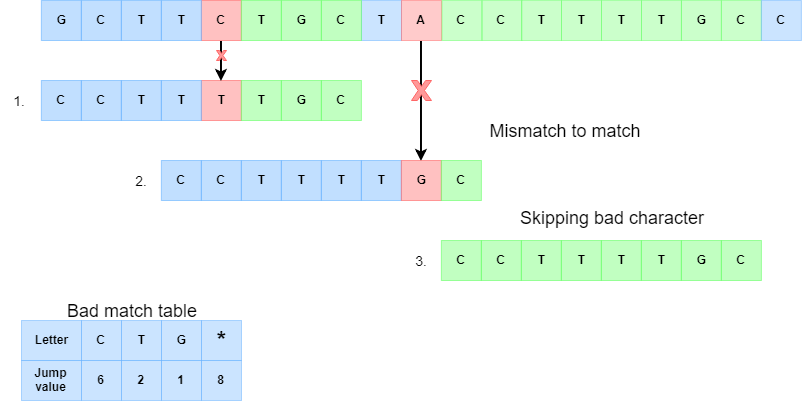
\includegraphics[width=\linewidth]{Images/BMBadMatch.png}
    \caption{Visualisation of the \acl{BM} bad match rule}
    \label{fig:BM_BadMatch}
\end{figure}
\newpage    
    \item Good Suffix: In searching the string when only a partial match is reached a search is then performed within the pattern to see if any sub-string of this partial match can exist in the pattern. 
\begin{figure}[!ht]
    \centering
    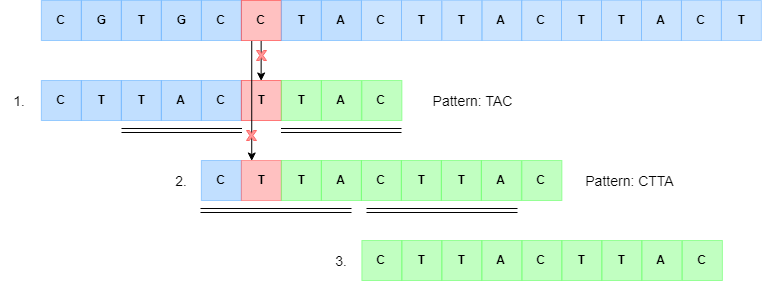
\includegraphics[width=\linewidth]{Images/BMGoodSuffix.png}
    \caption{Visualisation of the \acl{BM} good suffix rule}
    \label{fig:BM_GoodSuffix}
\end{figure}
\end{itemize}

When searching for a string \ac{BM}, typically, starts the patterns length into the string and reads patterns from their last character as they are discovered; right to left.
This can also be an issue as some of the patterns that are being searched for end with the default hex character on a empty disk {\textbackslash}x00.

As these jump tables are generated by \ac{BM} for each pattern, multiple searches through the string are required to find every pattern.
It would also be considered inefficient to implement BM into a functional algorithm for use on a GPGPU device for architectural difference to CPU that will be later explained. Due to GPGPU assets' much higher core count -- compared to CPU -- and independent memory a different approach to string searching is required to operate at a higher efficiency.

\subsubsection*{\acl{AC}}
The \acf{AC} method of string searching makes use of a pattern trees (tries) to navigate its search of many strings.
Using the state machine design from Knuth-Morris-Pratt, with said pattern tree, multiple strings can be searched for simultaneously.
This method results in almost no reduction in efficiency when attempting to search for multiple patterns.
\ac{AC} is also able to double back on itself within the tree where a pattern ceases but the potential of a different pattern exists; this functions similar to the good suffix rule previously discussed but would be better explained as a pointer to a different section of the search.
A visualisation of the jump table as explained can be seen in Figure \ref{fig:AC_diagram} will hopefully supplement the explanation.
\newpage
\begin{figure}[!ht]
    \centering
    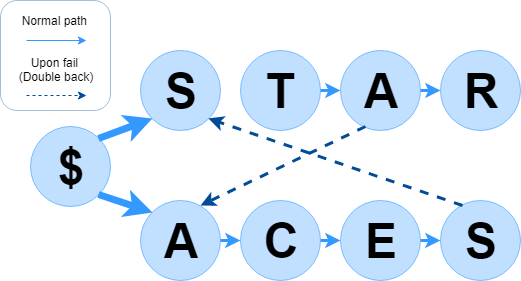
\includegraphics[width=240pt]{Images/AC_Visualisation.png}
    \caption{Visualisation of the \acl{AC}}
    \label{fig:AC_diagram}
\end{figure}
\subsubsection*{\acl{PFAC}}
\label{sec:PFAC}
\acf{PFAC} is the reduced version of \ac{AC}.
By removing the “Double Back” Failure states as seen in Figure \ref{fig:AC_diagram}, execution of the algorithm will simply cease in the event of a non-pattern.
This makes the algorithm more applicable for GPGPU architecture, where the intent would be to run the algorithm on many cores simultaneously and each thread of execution should remain as simple as possible.

\section{Research of current tools}
Before tests into the benefits provided by GPGPU methods can be developed, existing tools must be researched and a baseline must be established.
Unlike the methods in the paper ``Performance analysis of file carving tools’’ (Laurenson, 2013), the metrics being gathered for this will entirely be based on timings and data throughput.

Research for this investigation was focused into file carving tools that currently exist in open source; as these tools clearly showed how they operated.
Comparison between these tools allowed for great insight into favourable design practices, along with an understanding as to how the entire process of file carving is currently performed.
Analysis of these tools helped with identification into a platform to expand upon; although this decision concluded to not expand an existing platform but instead develop a new one for the purposes of testing.

From this and the literature that was reviewed, sufficient knowledge to develop this project was gained in the subject areas of; file carving, string searching, hardware and software design practices.
Multiple means of development were considered and one particularly difficult design choice was made during this stage between GPGPU \ac{API}s.

\subsubsection*{GPGPU Programming Libraries}
Before development could begin the choice of which \ac{GPGPU} \acf{API} should be used was considered.
This was between the options: CUDA or OpenCL.
This choice between the \acp{API} was made to ensure the right balance is being met between; ease of product development, delivery to multiple platforms, and \ac{API} performance.

The CUDA platform has the benefit of being simpler, thus easing product development, and having many optimisations as it is built for a specific subset of hardware.
The latter point comes with its disadvantages as CUDA is limited to Hardware distributed by NVidia.

The OpenCL platform is Open Source and developed for many hardware types which makes the final product more accessible, thus available to more systems.
Performance, although less efficient, can be made up from CUDA by making use of the \acf{IGP}.
The disadvantage here is in the time it will take to develop for this platform due to its complexity.

As such, it was decided that between these two platforms CUDA should be used and development of the final product was executed using this \ac{API}.

\section{Development}
Once the main body of research was complete and the foundation was decided upon, development could begin using C++ with the CUDA \ac{API}.
This language has its benefits in the researchers perspective due to previous knowledge of not only the syntax but of the and high efficiency the code can compile to meet.
As the existing tools, Scalpel and Foremost, make use of C and C++ they were used as a reference as to how to perform certain actions.
Furthermore, where these examples lacked, both C++ and the CUDA \ac{API} have readily available and verbose documentation -- not to mention large presences on Stack Overflow -- that could assist in the implementation process.

\subsubsection*{\acl{RAD}}
As it was expected that a great deal of time would be spent in the tool testing and development, this appeals to a methodology that makes use of proto\-typing.
As such the \acf{RAD} model was chosen. The \ac{RAD} methodology can be seen in Figure \ref{fig:RAD}.

\begin{figure}[!ht]
    \centering
    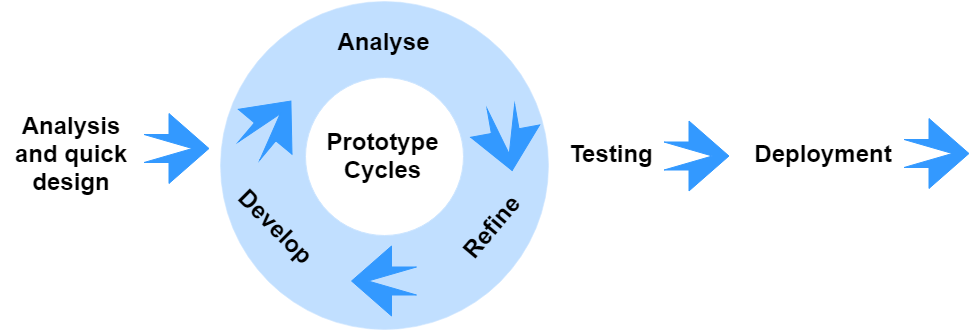
\includegraphics[width=230pt]{Images/RAD.png}
    \caption{\acl{RAD} Model}
    \label{fig:RAD}
\end{figure} 

By allowing testing to be performed during development, comparisons between all of the branches/prototypes test metrics would reveal where the development should continue.
This also subsequently helped to reveal many avenues of Future work.

\subsubsection*{Development environment setup} % These were used for the testing
In order to begin programming after decisions were made as to how to proceed, an environment was required that allowed for the compilation and execution of CUDA code.
CUDA makes use of it's own compiler, the NVidia C Compiler (NVCC), and although this can be installed without CUDA assets installed it is not typically recommended.
Two methods were employed to assist in the compilation and execution of CUDA code: NSight for Visual Studio (Windows) and the NVidia CUDA Toolkit (for Ubuntu).
Both of these had their merits as they each Operating system had tools that would be compared against that were native to them.

Each environments hardware specifications were taken to provide more insight and clarification as to the results of each test.
Tests that were made on one environment should not be compared to those from another due to the major differences that exist between them.
\acf{AWS} was used for testing to allow for the recreation of results.
By using this hardware/instance template any user should be able to access the same environment during their own testing.

{\centering
\begin{tabular}{c | c | c}
& Environment A & Environment B \\
& Personal Desktop & AWS g3s.xlarge \\
\hline
CPU & 4 Core, i5 3570k & 4 vCore's, Xeon E5-2686 v4 \\
\hline
GPU & GTX 980 Ti & TESLA M60 \\
\hline
Memory & 16\ac{GB}, 1333MHz & 30.5\ac{GB} \\
\hline
Backing Storage & \ac{SSD}, ?\ac{MB}/s & \ac{SSD}, 107\ac{MB}/s \\
\hline
\ac{OS} & Windows & Ubuntu Server 18.04 \\
\end{tabular}
\captionof{table}{Testing Environment Specifications}
\label{tab:TestingEnv}
\par}

Environment A's Backing storage speed is undetermined as the tool that was used to measure it returned improbable results for read speeds.
The given result suggested that reads could take place at 2483.00 MiB/s (2603.614 \ac{MB}/s) where the maximum theoretical bandwidth possible for a SATA III device is 600\ac{MB}/s.
These results were taken via the tool \href{https://github.com/Microsoft/diskspd}{diskspd.exe} and it is assumed that the developers really meant Megabits (Mb) which would result in 310.4MB/s.
This issue was clearly brought about by the inconsistent standard for what MiB stands for so the true limit of the disk was unestablished but the highest recorded speed was 390.27MB/s.

Now with access to the CUDA Compiler now established on two machines and their specifications known, implementation could proceed.

\subsubsection*{Implementation}
The development of the program was split into sections that could operate autonomously, thanks to the use of object oriented programming.
These compartmentalised sections were the file chunking method and the string searching method.
Both of these were designed independently due to the benefits that are provided when testing the code for both syntax and logical errors.
When searching for errors in the file chunking method this technique especially proved its worth but this will later be discussed.

The \ac{PFAC} string search was another key part of this implementation.
This search was designed through multiple iterations from single-threaded \ac{CPU} right up to multi-threaded \ac{GPU}.
The complete search could be identified as two different sections, the \ac{PFAC} search tree and the \ac{PFAC} search.
Referencing the OpenForensics code, written in C\#, this algorithm was implemented.

\section{Final Analysis}
Although analysis was performed throughout the development cycle the gained results were not not directly compared with other file carvers in a quantitative manner.
As such, the final analysis included direct comparisons between the final prototype and these existing file carvers while they are set to audit for files but not carve them.
This process took extra steps to accommodate the differences present between each tool analysis.

Test images were generated for this containing files known to the researcher.
As such the researcher was able to accurately test these tools for false positives and negatives as they knew exactly what results are to be expected with headers and footers.

After testing against other tools the processing rates of each chunk once it has been provided to the \ac{GPU} was subject to comparison followed by the data throughput.
Data Throughput of the program will be compared to the `theoretical maximum' (Bayne, 2017); the theoretical maximum in this context is in reference to the backing storage's ability to provide the data -- Disk Image Chunks –- to search.
This testing was performed multiple times to reduce the chance of `jitter' (Bellekens et al., 2017) effecting the results integrity.

As not all tools were able to be ran on the same system -- mostly due to the \ac{OS} compatibility of each – test results were only compared to other results on the same system.
Development as a result kept focus on the likely use on multiple devices and did not focus development to one system configuration.

% \section{Further Optimisations}
% Even during the process of development it was clear that some sections should be removed from the realm of expectation and assigned as future work.
% Only through complete trust of the theoretical design of the final product was this easy to distinguish.
% This is why much of the time distributed in this investigation was to gaining an understanding of existing file carvers.
% Many of these aspects that were future work however were items that could in fact easily be implemented.
% It is because of this optimisations were not expected to make it into the final product were able to be made throughout the development.
% Sections that were initally considered as future work will be discussed as they are discussed. % 1143 words
% Chapter 4 - Results
%   Tool Implementation
% 	Profiling final product
% 	Measuring the Hypothesis

%- Guide (250-1000 Words)

\chapter{Results}
\label{chap:chapter4}
To better explain each result the order that was described in the methodology section will not be followed.
First the implementation of the tool will be discussed, followed by issues encountered in development and finally comparisons between results from the Aletheia platform and existing file carving programs.

\section{Tool Implementation}
\label{sec:PFACResults}
As mentioned above in the methodology, implementation was split into two sections that worked together to become the final file header/footer search.
These two sections can be seen in the GitHub Repositories, \href{https://github.com/yeroc-sebrof/fileChunkingClass}{yeroc-sebrof/fileChunkingClass} and \href{https://github.com/yeroc-sebrof/Aletheia}{yeroc-sebrof/Aletheia}.
Development of the tool was performed through milestones as a staged development process, as expected of \acl{RAD}.
This iterative process was effective in the creation of the final tool.

The results from the \ac{CPU} versions of the tool show insight as to the improvement in not only the development of the tool but that comes with the use of \ac{GPGPU} methods.
When comparing these tools to the existing Foremost and Scalpel tools that are later tested it is clear to what extent the \ac{PFAC} algorithm is ill fitted to CPU execution.
Appendix \ref{sec:PFACappendix} contains said results from each main stage of the \ac{CPU} tools development as well as links to the code repositories.

\section{Evaluation of the final product}
\subsection{Selected File Types Searches}
\label{sec:fileTypeTest}
For testing the researcher relied on easy to generate file types.
The types that were tested for include: PNG, JPG, GIF, PDF, DOC and HTML.
File systems were then generated, of size 64\ac{MB} and these files were inserted within them to be searched for.
For this testing the chunk size for the file carver was reduced to search in 16\ac{MB} chunks.
All of these file systems tested individually against specifically compiled versions of Aletheia that would only search for the particular file type of each.

Appendix \ref{sec:fileTypeTestApp} contains the complete results of these simple tests but further testing was required due to unexpected false positives and negatives.
The encountered difficulties of false positives were acceptable; it can be considered common that stings that resemble a file header/footer can be found when they are not there for that reason.
\newpage
\subsubsection*{HTML problems}
\label{sec:HTMLissue}
Aletheias false negatives, which can be seen in Appendix \ref{subsec:fileTypeHTML}, were an issue that needed further exploration.
Due to the simplicity of this file type this issue was easy to trace.
Aletheia was modified to send the contents of the buffer where this footer should have been located to the console window.
As it can be seen in Figure \ref{fig:BadHTMLCout} this section of text did not appear as expected.

\begin{figure}[!ht]
    \centering
    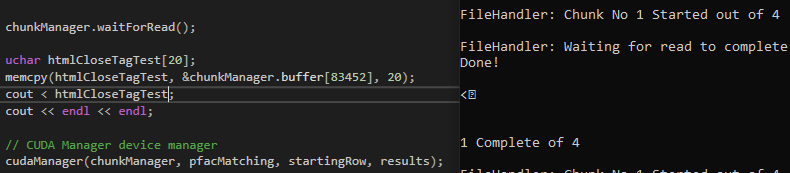
\includegraphics[width=\linewidth]{Images/Tests/64MB/MalformedClosingtag.png}
    \caption{Malformed Closing Tag}
    \label{fig:BadHTMLCout}
\end{figure}

As the pattern expected was \texttt{</html>} it was now clear why the footer was not found.
Further observation via the debug memory trace showed that the characters were not being read in correctly from the file.

\begin{figure}[!ht]
    \centering
    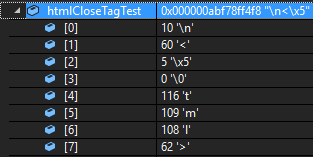
\includegraphics[width=200pt]{Images/Tests/64MB/MemoryRead.png}
    \caption{Memory Window}
    \label{fig:BadHTMLMem}
\end{figure}

Conclusions as to the source of this behaviour can be seen in the Discussion at Section \ref{subsec:fileTypeDiscussion}.

\subsection{Testing all File Types}
\label{sec:AllFileTypes}
Testing continued into searching for multiple documents through one file system of size 400\ac{MB}.
Two searches were performed but the patterns being searched for changed.
The results of this test were to determine if false positives were continuing and how many would occur in this simple example;
especially since a real world example would contain considerably more files.

The figures in Appendix \ref{sec:400MBAppendixPatterns} show the patterns that were enabled in each attempt.
This test was also able to show the speed difference obtained when less patterns were part of the search.
As you can see in Figure \ref{fig:runOnePatts}, run one was only reduced to search for patterns that could delay each thread of processing.

Overall, the tests ran without issue and the results were within expected parameters.
Said results from each run can be seen in Appendix \ref{sec:400MBAppendixResults}.

\subsection{Testing against a larger file system}
This next test was made with 10 PDFs spread out over a 2\ac{GB} disk image.
PDFs were chosen as they have been consistent to this point in returning only one header and footer.
First the disk was searched using only the PDF patterns loaded in Aletheia then the same disk image was compared to all of patterns the used in Figure \ref{fig:runOnePatts}, from the test of the 400 \ac{MB} disk.

The results that were gathered from this were very interesting and the conclusions drawn can be seen in the discussion in Section \ref{sec:400MBand2GBtookSimilarTimes}.

\subsection{Linux testing}
\label{sec:linuxResults}
All of the tests that were performed above, were then repeated on the second test environment to compare between.
The \ac{AWS} instance was used to then to provide a point of comparison to other, Linux bound, tools.

Although the \ac{SSD} was not optimal on Environment B, it was hoped that would be mitigated through the use of ram disks.
A ram disk is when a section of the main memory is assigned accessible in the same manner as backing storage drive.
Sections of testing showed that ram disks made a considerable difference to foremost but this was not a discernible difference as you can see from the results in Appendix \ref{sec:linuxTesting}, this did not have an effect on the data throughput.
Testing remained using ram disks however encase a noticeable difference could be later noticed.

Due to the shared tenancy of the \ac{AWS} instance there was an interesting set of results where the average time for the 2GB file searched for All patterns resulted in 24.512 seconds average per execution.
This test was performed again hours later for more accurate results.

\section{Comparisons to existing tools}
All of the following tests make use of the appropriate options/flags to disable the carving of the files.
These tools are only performing disk audits so the tasking is similar to Aletheias file header/footer search thus making it a fairer test.

\subsection{OpenForensics}
\label{sec:OpenForensicsComparison}
Although seldom mentioned up to this point, the only tool that was found in open-source that makes use of \ac{GPGPU} methods for file carving OpenForensics was used to compare against.
OpenForensics, authored by Dr Bayne is the testing platform mentioned in the paper ``Accelerating Digital Forensic searching through \ac{GPGPU} Parallel Processing Techniques'' (Bayne, 2017).

Testing on the 400\ac{MB} and 2\ac{GB} file showed that the tool can perform at incredibly high speed on both \ac{CPU} and \ac{GPU} (as well as amalgamations of the two).
Unfortunately, issues were experienced in trying to get the 10 \ac{GB} file over from Environment B for testing in time for the final round of testing on commercial hardware was not possible.
Moreover, this testing was very limited as to the number of runs performed due to the tool being GUI driven.

The results that were gathered can be further examined in Appendix \ref{sec:OpenForensicsAppendix} and the discussion in Section \ref{sec:OpenForensicsDiscussion}.

\subsection{Foremost \& Scalpel}
\label{sec:ForemostScalpelRes}
Although both Foremost and Scalpel have windows versions, it was very difficult to compile and believed that these tools would have to function in a Linux subsystem;
which would have caused significant performance reductions making testing unfair on Environment A.
On Environment B however, for testing to take place accurate only timing was required.

The GNU utility `time' was used to measure the speed of Scalpel and Foremost on the Linux platform to the millisecond.
This utility was unable to have the output piped to a file however so manual testing was reduced to 5 runs of each tool.
Both of these tools would have recorded their time own timings but only in Seconds, so not accurate enough for this test.
A comparison using the Aletheia platform was taken to examine the added overhead to tools due to this utility which can be seen in Appendix \ref{sec:overHeadApp}.
Aletheias results from Appendix \ref{sec:overHeadApp} were included in this comparison to ensure the test is fairer.
All of the Results from these tests can be seen in Appendix \ref{sec:SNFappendix}.\\

\subsubsection*{Foremost}
Although the patterns may be different between tools, all patterns were also used as a point of comparison.

Interestingly, in testing the tool more than once, between restarts, the tool exhibited significantly faster results after test one was performed.
This was expected to be some sort of caching within either the tool or the \ac{AWS} platform.
As a result between each test of the tool, the Ubuntu instance had to be reset to ensure accurate results. % 
%Chapter 5 - Discussion


%- Guide (1000-1500 Words)

\chapter{Discussion}
\label{chap:chapter5}

\section{Research Questions and Objectives}
The Research Question that fuelled this investigation was: `How much improvement can be made to the forensics file carving process using \ac{GPGPU} methods?'.
The Aim of this was to measure any achievable performance gain using both \ac{GPGPU} methods and modern algorithms for file carving.
It was also important to recognise any downfalls that come with using this process.

It is the researchers belief that, in looking back, the objectives that were set forth were met.
Said objective include:
\begin{itemize}[noitemsep, topsep=0pt]
    \item Locate and digest material from research of successful methods of improving performance with string searches for \ac{GPU}
    \item Implementing discovered methods to perform string searches on disks and memory
    \item Comparing all of the implementations in the above step with verbose testing
\end{itemize}

\subsection{Staged Development \ac{GPGPU}}
Through the course of the software development cycle, and following with the \ac{RAD} methodology, prototypes were created that gradually progressed the PFAC Algorithm to it's final iteration.
Each of these steps were also kept to integrate with the fileChunkingClass for comparison as can be seen in Section \ref{sec:PFACResults}.

This went through 4 main stages:
\begin{itemize}[noitemsep, topsep=0pt]
    \item PFAC compilation for a Single CPU core
    \item Having PFAC run across Multiple CPU cores in parrallel
    \item Getting PFAC to integrate with the CUDA types
    \item and successfully running PFAC accross the GPU
\end{itemize}

Moreover, throughout the development it was important to, where possible, optimise this process.
As the existing methods that exist would have been subject to multiple rounds of optimisation having a completely optimised final product would have paled the potential gains that could be obtained.
\newpage
\subsection{Unexpected Changes and Refinements}
Changes to the original scope were made in order to add focus to the research question during development.
The scope originally encompassed the idea that a full file carving program could be made in OpenCL.
This would have been optimal due to the -- previously discussed -- accessibility of OpenCL and to more clearly compare existing tools to the final product.

Through development it was made clear that the proposed scope would have been impossible within the allotted time to this research.
Many of the elements that would have allowed for this project to become a fully functioning file carver were left to future work.
Furthermore, research into the optimal methods to file carve each file type could have encompassed a dissertation within itself.

\section{Evaluation of Results}
\subsection{Individual File Type Test}
File types were searched for in this section individually to measure false positives and discover if each file would be found by the file search as intended.
The results contained in Section \ref{sec:fileTypeTest} and Appendix \ref{sec:fileTypeTestApp} show that the false positives existed but also showed that false negatives also were occurring.
The developer expected false positives at this time as the file carving element was not there to confirm the legitimacy of each result.
False negatives however were a big issue that should not of been occurring and were investigated.\\

\subsubsection*{False Negatives}
\label{subsec:fileTypeDiscussion}
As the HTML file footer was unable to be found and was simple enough to explore the researcher debugged the issue.
The \href{https://github.com/yeroc-sebrof/fileChunkingClass}{fileChunkingClass} was believed to be in error as characters were being fetched from the disk imaged incorrectly.
The hypothesis that the researcher came to is that the \texttt{\textbackslash} character was somehow escaping part of the unsigned character that was meant to be \texttt{h}.
Thus resulting in new required pattern to find the footer:

{\centering
\texttt{\{`<',{\textbackslash}x5,{\textbackslash}x0,`t',`m',`l',`>'\}}.
\par}

The result seen from using this new pattern can be seen in Appendix \ref{subsec:fileTypeHTML}.
This new HTML footer was not used in any other section for fairness when comparing later to other tools.

It was assumed from this that the false negatives from the other file types were due to similar circumstances.
As file carving was not to take place however, this was deemed an acceptable failure within the fileChunkingClass that would need to be resolved before expansion could be made into a file carving tool but for this purpose was acceptable.
The most important result from this testing is the data throughput and even though the false negatives could skew the final results this would be negligible in the researchers opinion.

\subsection{Full File Type Test}
Testing of all of the file types that were in use was performed against one file system of size 400MB.
Two tests were performed two different sets of patterns to search for; one set of patterns being a subsection of the other.
The final listing of file patterns used can be seen in Figures \ref{fig:runOnePatts} and \ref{fig:runTwoPatts}
This test both determined if false positives were continuing and how difference could be measured in time taken between different quantities of patterns.

As you can see in Figures \ref{fig:runOneResults} and \ref{fig:runTwoResults} the speeds differed, on average, by 32.46ms in the favour of the PFAC Table that contained all of the patterns.
This result was unexpected but due to the test being repeated 50x to achieve these were certainly the average speeds, these results can be seen in Table \ref{tab:WindowsTestingSumm400MB}.

This test did go on to prove that there is false positives for files that do not exist in this disk image but again this was expected;
it would be the job of a file carver to gain clarity though these false positives.

\subsection{2 \acl{GB} file with 10 PDFs}
\label{sec:400MBand2GBtookSimilarTimes}
This test was performed to collect more information regarding run speeds of the tool.
The consistent use of only PDF was to give the researcher a firm grasp as to how many files header/footers should have been discovered.
Tests were ran 50 time to confirm their validity with three different patterns loaded to compare.
Furthermore a comparison could be made between the 400\ac{MB} Test Two Patterns seen in Figure \ref{fig:runTwoResults} of Sub-Appendix \ref{sec:400MBAppendixPatterns} to better understand how the algorithm scales.

\subsection{Linux comparisons}
Finally for inter tool testing, the Linux version of the tool was tested using all of the available test images from Windows testing.
Linux was also able to generate a 4th test image of 10GB that was once again filled with PDFs that were randomly distributed throughout.
This all can be seen in Appendix \ref{sec:linuxTesting}.

The testing for this section was moved into a RAM disk.
This meant that instead of loading the files from a hard disk they were already in main memory.
A comparison to loading the files for the \ac{SSD} has been made as well within Sub-Appendix \ref{sec:aletheiaRamDisk}.

The results, as seen in Section \ref{sec:linuxResults} show that the Aletheia tool runs
\newpage
\section{Comparison to Existing Tools} % What can they do better? are they trash? does it not work on the platforms or in the scale i want?
\label{sec:existingTools}

\subsection{OpenForensics}
\label{sec:OpenForensicsDiscussion}
OpenForensics was developed alongside the aforementioned paper ``Accelerating Digital Forensic searching through \ac{GPGPU} Parallel Processing Techniques'' (Bayne, 2017).
This tool, using OpenCL, can make use of \ac{GPGPU} and \ac{CPU} assets simultaneously which was seen during the testing stage along with just \ac{GPU}.
Furthermore, for the purpose of fair testing this tool is also able to search for individual file types so testing was performed with both: PDF only and All types.

As seen in Section \ref{sec:OpenForensicsComparison} OpenForensics, clearly due to it more established and tested status, runs better than the Aletheia platform.
In itself this further proves the research question by showing how much improvement there stands to be gained against existing file carving tools.

\subsection{Foremost \& Scalpel}
As it can be seen from the results in Section \ref{sec:ForemostScalpelRes} Foremost was difficult to test due to the interesting results that were accumulated.
Testing the tool once before restarting the \ac{AWS} instance resolved this issue to increase the accuracy of results.
However this greatly increased the time taken to collect results so less total results could be added to fortify the average run time in Appendix \ref{sec:SNFappendix}.

It was interesting how pronounced the time differences imposed by \acl{BM} became when making use of only one pattern as a comparison to all patterns.
But due to the fact the search would need to be performed again for each pattern, this was unsurpirsing.

In comparing the Aletheia platform to these established tools the speed difference in the favour of Aletheia was gratifying.
This also solidified the answer to the research question -- ``How much improvement can be made to the forensics file carving process using \ac{GPGPU} methods?'' -- and quantified it via the test cases to up to a factor of 15x (When comparing Table \ref{tab:AverageScalpelAllPatt} to \ref{tab:UbuntuTestingSumm2GBRAM} with the All patterns for the 2GB file).
\newpage
\section{How existing tools can be improved using \ac{GPGPU} acceleration}
Using both the speeds that were accumulated from OpenForensics and Aletheia it is clear that improvements can be made on the Foremost and Scalpel platforms.
The OpenForensics platform even shows that through the correct use of resource management on the \ac{CPU} can be vastly improved and search times, in comparison to single threaded tools, can be multiplied by at least the sum of the concurrent cores.
With the new generations of hardware that are being released core counts are being greatly increased\footnotemark and processing speed on CPU could go with it.
\footnotetext{AMD Ryzen Threadripper 2990WX Processor, 32 Cores\\ \href{https://www.amd.com/en/products/cpu/amd-ryzen-threadripper-2990wx}{https://www.amd.com/en/products/cpu/amd-ryzen-threadripper-2990wx}}
Although the idea of having thousands of GPU cores outperformed does not seem possible, the time saved on the memory copies could see this as possible with enough threads of execution.

From the implementation of the Aletheia platform the multiple buffers that exist on the \ac{CPU} and the \ac{GPU} having their own memory spaces has both pros and cons.
Being able to synchronously load in a chunk to one buffer while reading another was a useful design.
This could be easily replicated on \ac{CPU} devices, it also does not need to be limited to simply 2 buffers.
The idea of having multiple buffers could come in use to carve during the searching through file chunks, but this potential method would have its limits.

Even if none of the previous recommendations are implemented, by phasing out the use of \acf{BM} for file searching great boosts can be seen in performance.
\ac{BM} in it's ability to only read for a single pattern at a time is far out-shined in performance compared to the \acf{AC} algorithm.
As \ac{AC} is able to search for multiple patterns simultaneously the need for multiple search passes is completely removed.
This one change in itself could save considerable time in execution.
 % 

%- What conclusions can you draw from your investigation?
%- What are the implications of what you have discovered?
%- How might further work in this area be continued?
%- Guide -750 - 1000 words

\chapter{Conclusion}
In conclusion, the results seen from the \acl{GPGPU} header/footer search compared to both Scalpel and Foremost far exceed the expectations of the researcher.
Initial expectations were that processing would have increased by roughly a factor of 5.
Moreover, said expectations were that the contents of this research could be applied to a full file carver as a final product.

After the scope was reduced to conform with the time available, research was then limited to the creation of a file header/footer searching platform; named Aletheia after the translated Ancient Greek for ``truth or disclosure in philosophy''.
Through testing it was shown that the speed at which file header/footer searches far exceed that of CPU tools.
In one example, this difference was measured at 15 times greater data throughput when compared to the Scalpel platform.
The differences between these platforms are believed to be adequately drawn out and discussed through this investigation;
not only for the purpose of understanding the downfalls of the CPU tools but for setting up an adequate comparison.
Improvements that could be made to these platforms have also been discussed.

Development in this, somewhat niche, field of computing science is very important to not only the researcher but for law enforcement organisations.
Although file carving abilities were not developed, due to being out of scope, it is hoped that the file search that was developed through this research could be continued into another functioning, open-source file carver that is available to Digital Forensics investigators.
Access to a wider array of tools can be very important for not only confirmation of evidence but also for continued support in driving growth within the sector.
It is hoped that with more research into this subject area that the ever growing divide between digital crime and digital forensics will recede, even if just temporarily.
\newpage
\section{Future Work}
\subsubsection*{Continuous Development to Aletheia}
The work that was put into the implementation of the Aletheia platform could still be subject to improvement.
The developer has many areas they would wish to expand their work but it can be reduced to the following few points.

Solving the issues in Section \ref{sec:HTMLissue} would be a big step in ensuring the integrity of results for future iterations.
Looking into the existing Scalpel and Foremost codebases' would provide great insight as to what elements were poorly designed in the fileChunkingClass.
Following this it would be good to optimise the existing code and/or the include file carving elements.

It would also be useful to have the tool dynamically adjust to the environment that the tool finds itself in.
Aletheia could be configured to adjust itself to the GPU dynamically allocating GPU processor block sizes and to (V)RAM by allocating memory buffers.

Finally adding run time options along with general usability comparable to existing platforms would be a useful edition.
Being able to define the program behaviour without redefining the program would be of great use.

\subsubsection*{OpenCL}
With the knowledge from this paper and the existing code base, an OpenCL variant of the platform could be implemented.
Depending on the syntax differences or even a possible equivalent to Cudafy.net for C++, the existing code could potentially be adjusted to conform the OpenCL library.
This would hopefully also continue to attempt execution on multiple platforms.

\subsubsection*{Memory forensics}
The concepts from this research or the Aletheia platforms itself could be adjusted to be used in a Memory Forensics environment.
Real time monitoring of Virtual Machine RAM contents could be executed in the event the platform was able to perform quick enough.

% switch to two-column layout

\begin{multicols}{2}
{\small
\section*{Acronyms}
\subsubsection*{File Sizes:}
\acf{MB}\\
\acf{GB}\\
\acf{TB}
\subsubsection*{Hardware types:}
\acf{HDD}\\
\acf{SSD}\\
\acf{CPU}\\
\acf{GPU}\\
\acf{GPGPU}\\
\acf{IGP}
\columnbreak
\subsubsection*{Algorithms:}
\acf{BM}\\
\acf{AC}\\
\acf{PFAC}
\subsubsection*{Other:}
\acf{RAD}\\
\acf{IDS}\\
\acf{OS}\\
\acf{API}\\
\acf{AWS}
\par}
\end{multicols}

%now enable appendix numbering format and include any appendices
\chapter{Appendicies}
\renewcommand{\thesection}{\Alph{section}}
\section{Iterations of the PFAC algorithm}
\label{sec:PFACappendix}

\subsection{Code}
Overall the code that drive the Aletheia Header/Footer search can be seen in the final Git hub project:
\underline{\href{https://github.com/yeroc-sebrof/Aletheia}{here}} or through the link https://github.com/yeroc-sebrof/Aletheia

The code that contains the fully integrated CPU method is contained within a folder within the Aletheia Git hub project;

\href{https://github.com/yeroc-sebrof/Aletheia/blob/master/Prod/Previous/MultiCPU.cpp}{yeroc-sebrof/Aletheia/blob/master/Prod/Previous/MultiCPU.cpp}

This code currently runs on multiple CPU threads.
This method was able to be run in a single thread also by un-commenting line 181 and 203, and commenting line 177, 178, 183, 184, 189, 199, 200, 205, 206, and 211.

\subsection{Results}
Due to the time taken for this search on the CPU it was deemed reasonable to conduct the tests with a smaller number of run times.
Testing of the single threaded PFAC file header search was extremely slow and was only run twice to confirm the first result given.
The multi-threaded PFAC search obviously improved upon this design and was able to demonstrate performance gains.
This was only run run 10 times however.

The test here makes use of the 400MB test case from Section \ref{sec:AllFileTypes} and can be compared to the results in \ref{sec:400MBAppendixResults}.
Test results averaged to: 

{\centering
\begin{tabular}{c | c | c}
400 MB & Milliseconds & MB/s \\
\hline
PDF Only & 542507 & 3.69 \\
All Files & 108455.2 & 0.74 \\
\end{tabular}
\captionof{table}{Windows Single CPU Results 400MB}
\label{tab:windowsTestSingleCPU}
\par}



{\centering
\begin{tabular}{c | c | c}
2 GB & Milliseconds & MB/s \\
\hline
PDF Only & 35661.8 & 11.22 \\
All Files & 156529.4 & 2.56 \\
\end{tabular}
\captionof{table}{Windows Multi CPU Average Results 400MB}
\label{tab:windowsTestMultiCPU}
\par}

Throughput was measured using the standard $s = \dfrac{d}{t}$
 % CPU Test - 400MB
\newpage
\section{Results of the individual file type tests (64MB)}
\label{sec:fileTypeTestApp}

\begin{figure}[!ht]
    \centering
    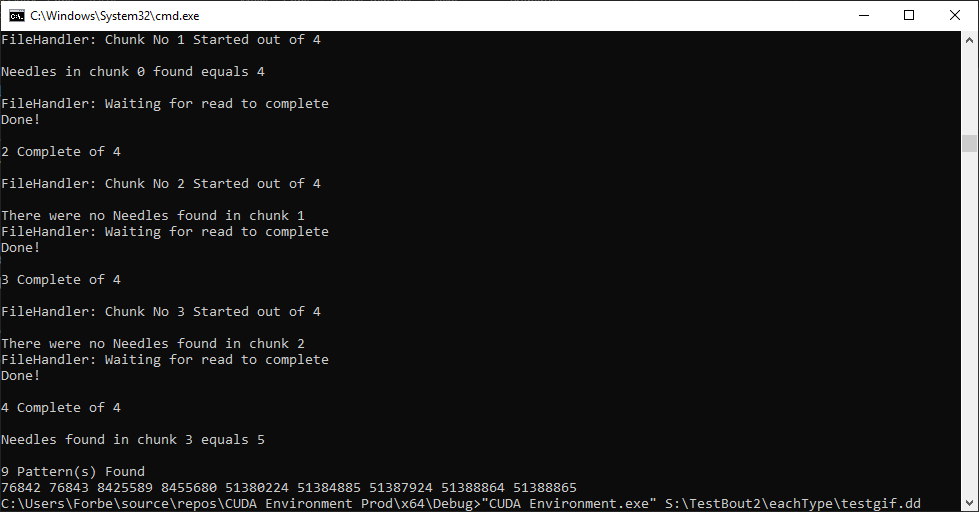
\includegraphics[width=\linewidth]{Images/Tests/64MB/GIFResult.png}
    \caption{Results from searching for .gif}
    \label{appItem:GIFsearch}
\end{figure}
\begin{figure}[!ht]
    \centering
    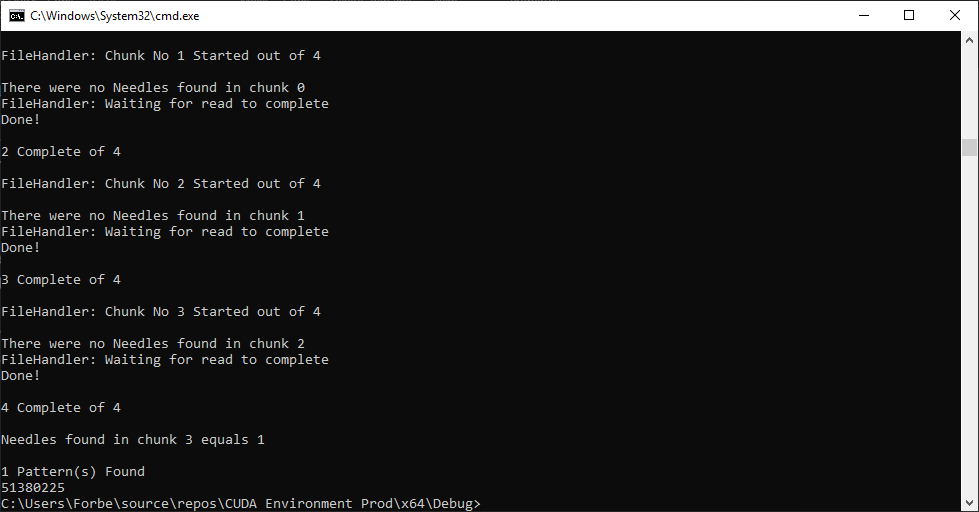
\includegraphics[width=\linewidth]{Images/Tests/64MB/PNGResults.png}
    \caption{Results from searching for .png}
    \label{appItem:PNGsearch}
\end{figure}
\newpage
\begin{figure}[!ht]
    \centering
    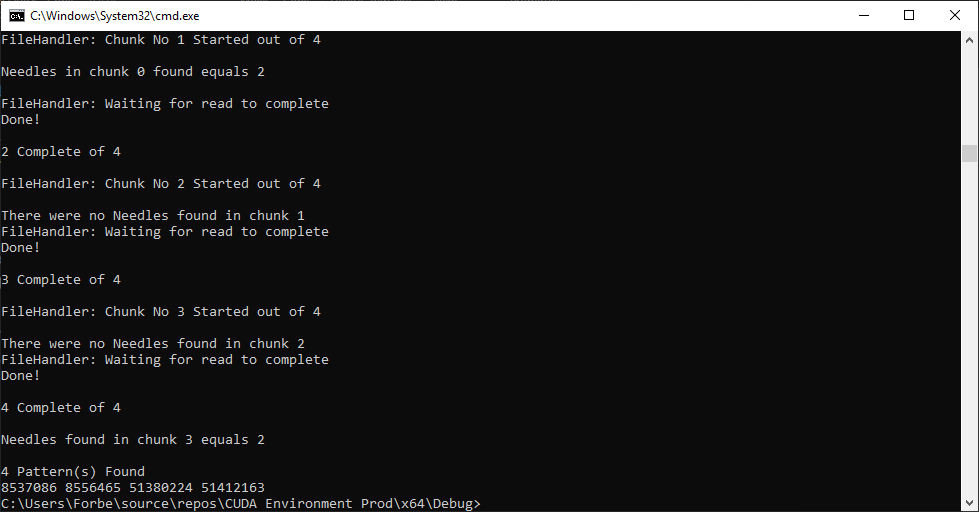
\includegraphics[width=\linewidth]{Images/Tests/64MB/JPGResults.png}
    \caption{Results from searching for .jpg}
    \label{appItem:JPGsearch}
\end{figure}
\begin{figure}[!ht]
    \centering
    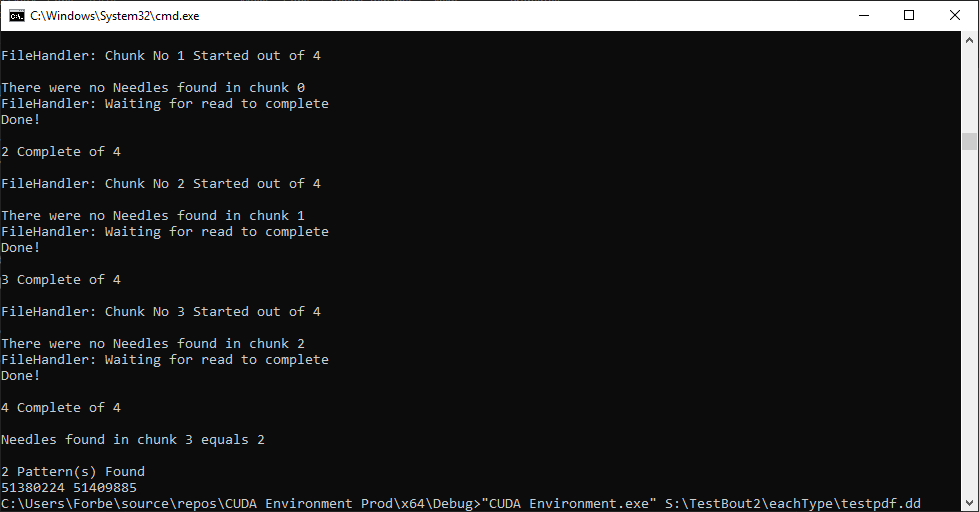
\includegraphics[width=\linewidth]{Images/Tests/64MB/PDFResults.png}
    \caption{Results from searching for .pdf}
    \label{appItem:PDFsearch}
\end{figure}
\newpage
\begin{figure}[!ht]
    \centering
    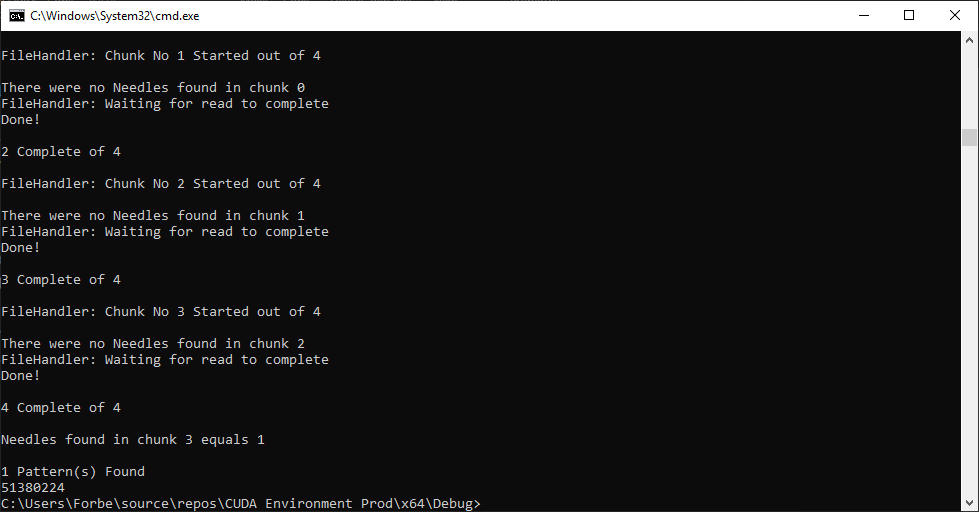
\includegraphics[width=\linewidth]{Images/Tests/64MB/DocResults.png}
    \caption{Results from searching for .doc}
    \label{appItem:DOCsearch}
\end{figure}
\newpage
\subsection*{HTML}
\label{subsec:fileTypeHTML}
\begin{figure}[!ht]
    \centering
    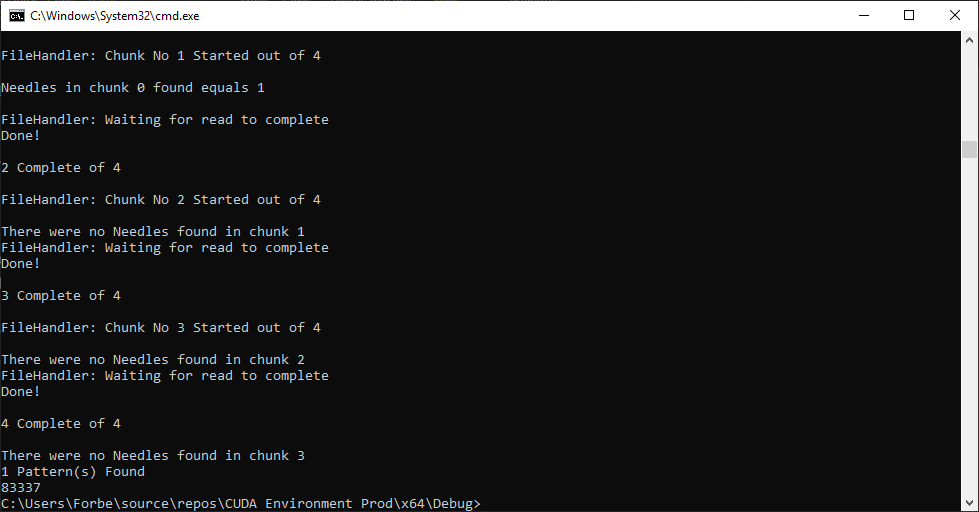
\includegraphics[width=\linewidth]{Images/Tests/64MB/HTMLResultORGFOOT.png}
    \caption{Results from searching for .HTML with original Foot Pattern}
    \label{appItem:HTMLsearchOLD}
\end{figure}
\begin{figure}[!ht]
    \centering
    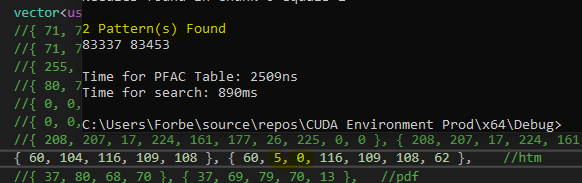
\includegraphics[width=\linewidth]{Images/Tests/64MB/HTMLResultnewFOOT.png}
    \caption{Results from searching for .HTML with new Foot Pattern}
    \label{appItem:HTMLsearchNEW}
\end{figure}
 % GPU tests of 64MB
\section{Results from the all file-types test (400MB)}
\subsection{Patterns}
\label{sec:400MBAppendixPatterns}
\begin{figure}[!ht]
    \centering
    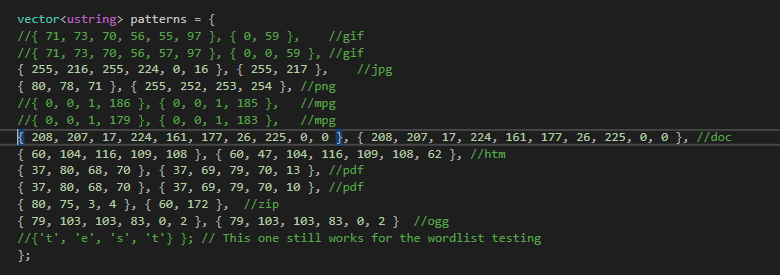
\includegraphics[width=\linewidth]{Images/Tests/2GB/Aletheia-Patts.png}
    \caption{400\ac{MB} Reduced \ac{PFAC} Patterns (Run One)}
    \label{fig:runOnePatts}
\end{figure}
\begin{figure}[!ht]
    \centering
    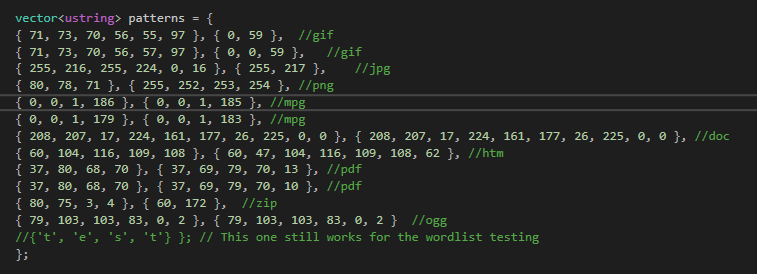
\includegraphics[width=\linewidth]{Images/Tests/400MB/runTwoPatt.png}
    \caption{400\ac{MB} All \ac{PFAC} Patterns (Run Two)}
    \label{fig:runTwoPatts}
\end{figure}
\newpage
\subsection{Results}
\label{sec:400MBAppendixResults}
\begin{figure}[!ht]
    \centering
    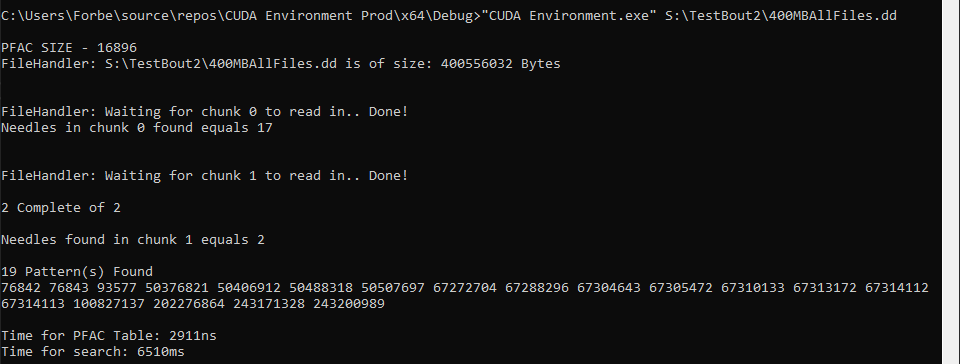
\includegraphics[width=\linewidth]{Images/Tests/400MB/runOne.png}
    \caption{400\ac{MB} Reduced \ac{PFAC} Patterns Results (Run One)}
    \label{fig:runOneResults}
\end{figure}
\begin{figure}[!ht]
    \centering
    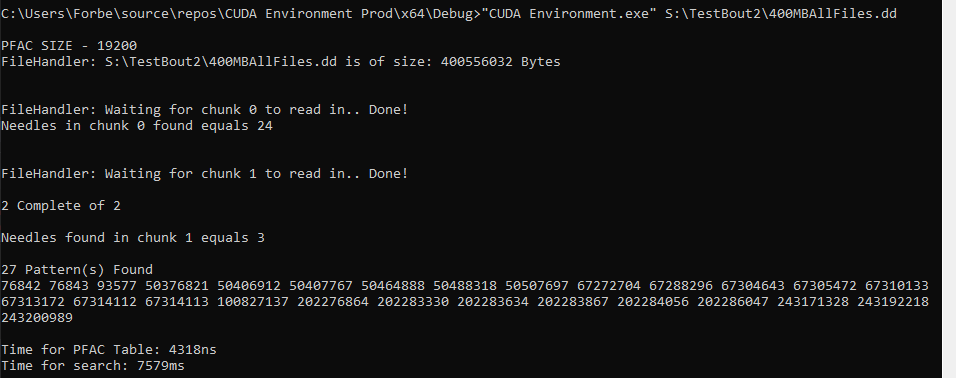
\includegraphics[width=\linewidth]{Images/Tests/400MB/runTwo.png}
    \caption{400\ac{MB} All \ac{PFAC} Patterns Results (Run Two)}
    \label{fig:runTwoResults}
\end{figure}

Averaged results from the above tests can be seen in Table \ref{tab:WindowsTestingSumm400MB} from Appendix \ref{sec:WindowsTesting}
 % GPU test of 400MB
\section{Results from the 10 PDF test (2GB)}

\begin{figure}[!ht]
    \centering
    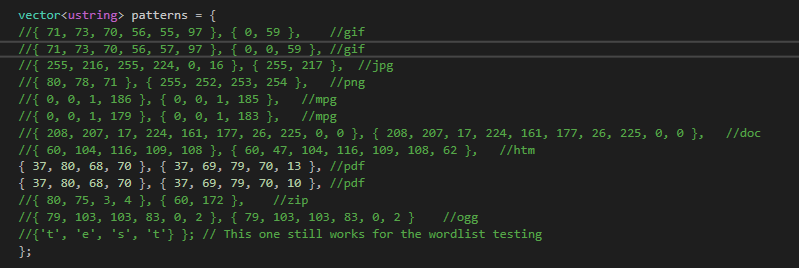
\includegraphics[width=\linewidth]{Images/Tests/2GB/Aletheia-PDF-Patts.png}
    \caption{\ac{PFAC} Patterns being searched for in 2GB file}
    \label{fig:2gbPFACPatterns}
\end{figure}
\begin{figure}[!ht]
    \centering
    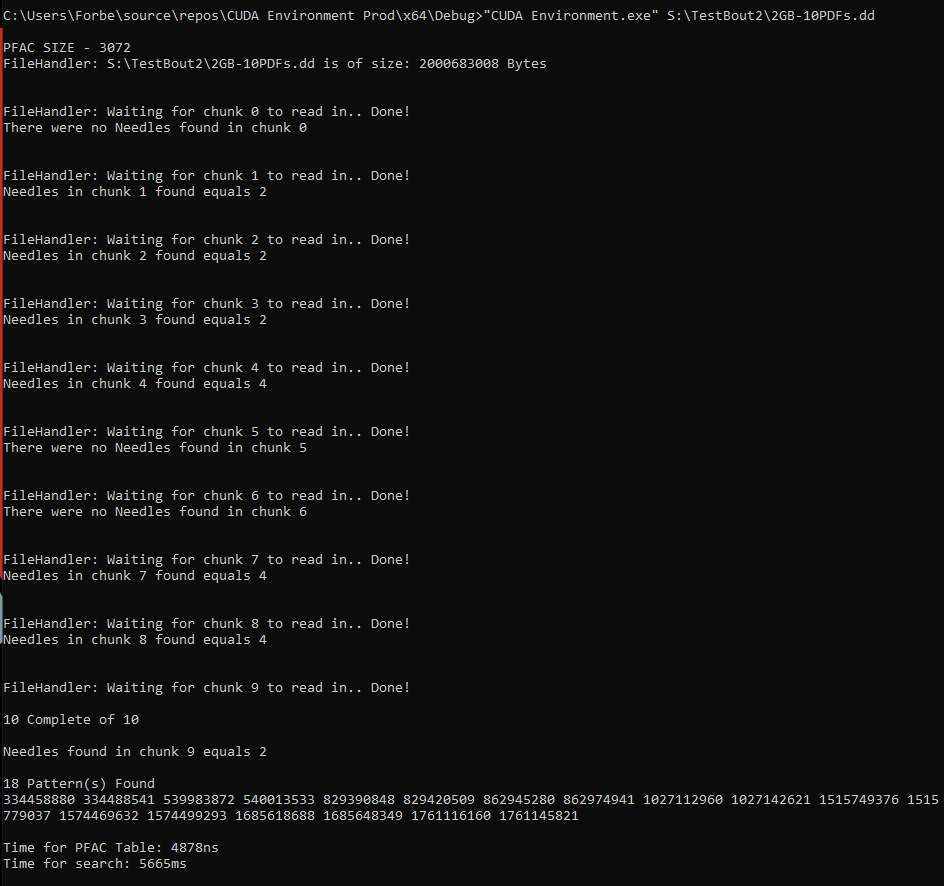
\includegraphics[width=\linewidth]{Images/Tests/2GB/Aletheia-PDF-Only.png}
    \caption{2\ac{GB} PDF only \ac{PFAC} Patterns Results}
    \label{fig:2gbPFACResults}
\end{figure}
\newpage
\begin{figure}[!ht]
    \centering
    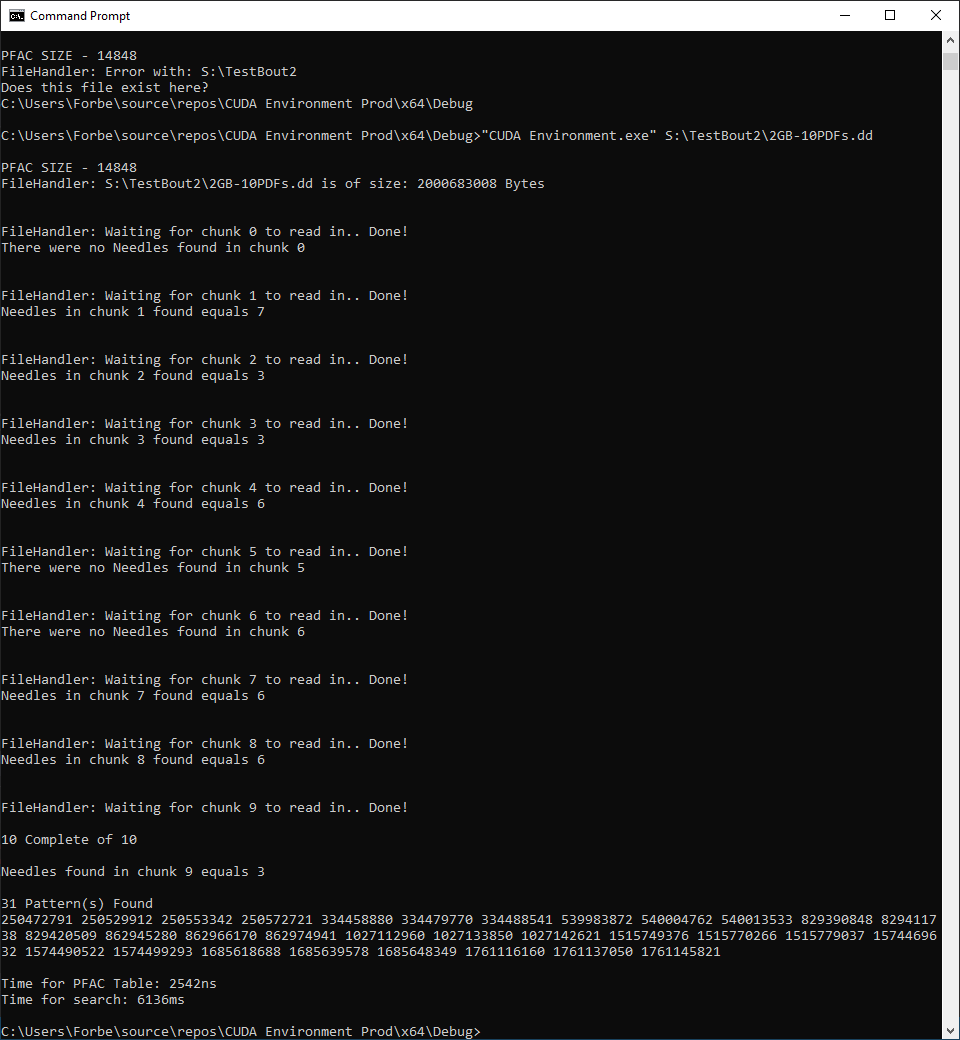
\includegraphics[width=\linewidth]{Images/Tests/2GB/Aletheia.png}
    \caption{2\ac{GB} \ac{PFAC} Patterns Results}
    \label{fig:2gbPFACResultsMore}
\end{figure}
 % 2GB
\section{Open Forensics Results}
\label{sec:OpenForensicsAppendix}

The results that were collected can be seen below


{\centering
\begin{tabular}{c | c | c}
2GB & Seconds & Mb/s \\
\hline
CPU & 4.81s & 416.18 \\
CPU PDF & 1.45s & 1381.65 \\
GPU & 1.3s & 1540.58 \\
GPU PDF & 1.16s & 1716.98 \\
\end{tabular}
\captionof{table}{Open Forensics running through the 2GB file}
\label{tab:OpenForensics2GB}
\par}

The speeds listed above appear to be Mb/s, and are listed as such, compared to MB/s as they are listed in each occurrence.
\newpage

\begin{figure}[!t]
\texttt{\input{Appendices/10PDFOpenForensics/CPUALLLogFile.txt}}
\caption{CPU Open Forensics All patterns 2GB File}
\label{fig:OF2CPUAllPat}
\end{figure}
\newpage
\begin{figure}[!t]
\texttt{\input{Appendices/10PDFOpenForensics/GPUALLLogFile.txt}}
\caption{GPU Open Forensics All patterns 2GB File}
\label{fig:OF2GPUAllPat}
\end{figure}
\newpage
\begin{figure}[!t]
\texttt{\input{Appendices/10PDFOpenForensics/CPUPDFONLYLogFile.txt}}
\caption{Open Forensics PDF patterns 2GB File}
\label{fig:OF2CPUPDF}
\end{figure}
\newpage
\begin{figure}[!t]
\texttt{\input{Appendices/10PDFOpenForensics/GPUPDFONLYLogFile.txt}}
\caption{Open Forensics All patterns 2GB File}
\label{fig:OF2GPUPFD}
\end{figure}
  %2GB
\section{Overhead from `time' utility}
\label{sec:overHeadApp}
The following table compares the results from the tests on Aletheia with and without the GNU tool.

{\centering
\begin{tabular}{c | c | c | c}
Aletheia & PDF & No Gif/mpg & All Files \\
\hline
GNU Time & 5791 ms & 5781 ms & 6254 ms \\
No GNU Time & 5481.78 & 5536.78 & 6006.96 \\
Diff & 309 ms & 245 ms & 247 ms \\
Increase & 17.75\% & 22.63\% & 24.3\% \\
\end{tabular}
\captionof{table}{GNU Time Differences}
\label{tab:GNUtimeDiff}
\par}

\section{Foremost and Scalpel tests}
\label{sec:SNFappendix}
Tests here were ran 5 times each due to issues with automating recording of resutlts.
Throughput was measured using the standard $s = \dfrac{d}{t}$

\subsection{Scalpel}
{\centering
\begin{tabular}{ c | c | c }
All Types & Time Taken & MB/s \\
\hline
Scalpel 2GB & 89726 ms & 22.29 \\
Scalpel 400MB & 16549 ms & 24.17 \\
\end{tabular}
\captionof{table}{Scalpel Average Results All patterns}
\label{tab:AverageScalpelAllPatt}
\par}

{\centering
\begin{tabular}{ c | c | c }
PDF only & Time Taken & MB/s \\
\hline
Scalpel 2GB & 12874 ms & 155.35 \\
Scalpel 400MB & 2978 ms & 134.33 \\
\end{tabular}
\captionof{table}{Scalpel Average Results PDF patterns}
\label{tab:AverageScalpelPDFPatt}
\par}

\subsection{Foremost}
{\centering
\begin{tabular}{ c | c | c }
All Types & Time Taken & MB/s \\
\hline
Foremost 2GB & 54498 ms & 36.70 \\
Foremost 400MB & 10941 ms & 36.56 \\
\end{tabular}
\captionof{table}{Foremost Average Results All patterns}
\label{tab:AverageForemostAllPatt}
\par}

{\centering
\begin{tabular}{ c | c | c }
PDF only & Time Taken & MB/s \\
\hline
Foremost 2GB & 17850 ms & 112.04 MB \\
Foremost 400MB & 2831 ms & 141.29 MB \\
\end{tabular}
\captionof{table}{Foremost Average Results PDF patterns}
\label{tab:AverageForemostPDFPatt}
\par}

%\section{Foremost and Scalpel tests}
\label{sec:SNFappendix}
Tests here were ran 5 times each due to issues with automating recording of resutlts.
Throughput was measured using the standard $s = \dfrac{d}{t}$

\subsection{Scalpel}
{\centering
\begin{tabular}{ c | c | c }
All Types & Time Taken & MB/s \\
\hline
Scalpel 2GB & 89726 ms & 22.29 \\
Scalpel 400MB & 16549 ms & 24.17 \\
\end{tabular}
\captionof{table}{Scalpel Average Results All patterns}
\label{tab:AverageScalpelAllPatt}
\par}

{\centering
\begin{tabular}{ c | c | c }
PDF only & Time Taken & MB/s \\
\hline
Scalpel 2GB & 12874 ms & 155.35 \\
Scalpel 400MB & 2978 ms & 134.33 \\
\end{tabular}
\captionof{table}{Scalpel Average Results PDF patterns}
\label{tab:AverageScalpelPDFPatt}
\par}

\subsection{Foremost}
{\centering
\begin{tabular}{ c | c | c }
All Types & Time Taken & MB/s \\
\hline
Foremost 2GB & 54498 ms & 36.70 \\
Foremost 400MB & 10941 ms & 36.56 \\
\end{tabular}
\captionof{table}{Foremost Average Results All patterns}
\label{tab:AverageForemostAllPatt}
\par}

{\centering
\begin{tabular}{ c | c | c }
PDF only & Time Taken & MB/s \\
\hline
Foremost 2GB & 17850 ms & 112.04 MB \\
Foremost 400MB & 2831 ms & 141.29 MB \\
\end{tabular}
\captionof{table}{Foremost Average Results PDF patterns}
\label{tab:AverageForemostPDFPatt}
\par}
 % 400MBand 2GB

\section{Results from repeated testing -- Windows}
\label{sec:WindowsTesting}
Tests were repeated here for 50 runs and have been averaged using a mean average.
Throughput was measured using the standard $s = \dfrac{d}{t}$

{\centering
\begin{tabular}{c | c | c}
400 MB & Milliseconds & MB/s \\
\hline
All Patterns & 1760.7 & 227.18 \\
All Files & 1728.24 & 231.45 \\
PDF Only & 1711.44 & 233.72 \\
\end{tabular}
\captionof{table}{Windows Results 400MB}
\label{tab:WindowsTestingSumm400MB}
\par}

{\centering
\begin{tabular}{ c | c | c }
2GB & Milliseconds & MB/s \\
\hline
All Patterns & 5436.15 & 376.74 \\
All Files & 5247.6 & 390.27 \\
PDF Only & 5776.4 & 354.55 \\
\end{tabular}

\captionof{table}{Windows Results 2GB}
\label{tab:WindowsTestingSumm2GB}
\par}

\newpage
\section{Results from repeated testing -- Ubuntu}
\label{sec:linuxTesting}
Tests were repeated here for 50 runs and have been averaged using a mean average.
Throughput was measured using the standard $s = \dfrac{d}{t}$

\subsection{Ubuntu SSD}
{\centering
\begin{tabular}{ c | c | c }
2GB & Time Taken & MB/s \\
\hline
PDF Only & 5481.78 & 373.60 \\
"Files that exist" & 5536.78 & 369.89 \\
%All files & 24512.76 & 83.5483234 \\
All files & 6025.65 & 339.88 \\
\end{tabular}
\captionof{table}{Ubuntu Average Results 2GB SSD}
\label{tab:UbuntuTestingSumm2GBSSD}
\par}

\subsection{Ubuntu Ram-Disk}
\label{sec:aletheiaRamDisk}
{\centering
\begin{tabular}{ c | c | c }
400MB & Time Taken & MB/s \\
\hline
PDF Only & 3057.73 & 130.82 \\
Files that exist & 2893.54 & 138.24 \\
All files & 2893.54 & 130.39 \\
\end{tabular}
\captionof{table}{Ubuntu Average Results 400MB RAM}
\label{tab:UbuntuTestingSumm400MBRAM}
\par}

{\centering
\begin{tabular}{ c | c | c }
2GB & Time Taken & MB/s \\
\hline
PDF Only & 5481.78 & 373.60 \\
"Files that exist" & 5536.78 & 369.89 \\
All files & 6006.96 & 340.94 \\
\end{tabular}
\captionof{table}{Ubuntu Average Results 2GB RAM}
\label{tab:UbuntuTestingSumm2GBRAM}
\par}

{\centering
\begin{tabular}{ c | c | c }
10GB & Time Taken & MB/s \\
\hline
PDF Only & 24512.76 & 417.74 \\
FIles that exist & 24496.72 & 418.02 \\
All files & 24501.12 & 417.94 \\
\end{tabular}
\captionof{table}{Ubuntu Average Results 10GB RAM}
\label{tab:UbuntuTestingSumm10GbRAM}
\par} % All others
%\include{Appendices/appendixTestDiskCode}

%uncomment next line to change bibliography name to references
%\renewcommand{\bibname}{References}
%\bibliography{bibliography} %use a bibtex bibliography file refs.bib
%\bibliographystyle{agsm} %use the plain bibliography style
\chapter*{References}
Bayne, E. (2017) Accelerating digital forensic searching through GPGPU parallel processing techniques. Abertay University.

Bellekens, X., Tachtatzis, C., Atkinson, R., Renfrew, C. and Kirkham, T. (2017) 'GLoP: Enabling Massively Parallel Incident Response Through GPU Log Processing', 2014-. doi: 10.1145/2659651.2659700.

Jacob, N. and Brodley, C. (2006) Offloading IDS Computation to the GPU.

Laurenson, T. (2013) Performance analysis of file carving tools.

Marziale, L., Richard, G.G. and Roussev, V. (2007) 'Massive threading: Using GPUs to increase the performance of digital forensics tools', Digital Investigation, 4, pp. 73-81. doi: 10.1016/j.diin.2007.06.014.

Škrbina, N. and Stojanovski, T. (2012) 'Using parallel processing for file carving'.

\end{document}

